\section{Bahnführungsebene}
\label{ch_Bahnführungsebene}
Wie in Kapitel \ref{ch_3EM} bereits dargestellt, ist die Aufgabe der Bahnführungsebene die Realisierung verschiedenster Manöver,  definiert durch die jeweils darzustellende Kundenfunktion, wie z.B.  Spurhalten, Ausweichen, einem Vorderfahrzeug folgen, eine bestimmte Geschwindigkeit erreichen. 
Zur Umsetzung dieser Manöver wird häufig auf rein regelungsbasierte Ansätze gesetzt. Dabei ist meist der Regler an die jeweilige Fahraufgabe bzw.  Fahrsituation anzupassen bzw. zwischen verschiedenen Regelungsansätzen umzuschalten.  Eine sehr generische Lösung, die für verschiedene Fahrfunktionen verwendbar ist,  stellen dagegen trajektorienbasierte Ansätze auf der Bahnführungsebene dar.
\subsection{Trajektorienplanung}
Die Umsetzung der Manöver der Bahnführungsebene mittels einer Trajektorienplanung stellt mittlerweile eine weitverbreitete Methode dar (vgl.  \cite{Werling2016b}).  Die zu berechnenden Trajektorien müssen verschiedenen Anforderungen genügen: so muss zunächst die Sicherheit gewährleistet werden.  Die berechnete Bewegung muss stets kollisionsfrei mit anderen Verkehrsteilnehmern und Hindernissen sein. Zusätzlich sind Güteaspekte wie maximal auftretende Rücke und Beschleunigungen einzuhalten bzw. zu minimieren. Dies ist nicht nur aus Komfortaspekten zu tun sondern auch um die Bewegung durch die verwendete Aktuatorik realisieren zu können. Dazu muss das Potenzial des Antriebs bzw. der Lenkung und der verfügbare Reibwert berücksichtigt werden. 

%\begin{itemize}
%\item Anforderungen: 
%\begin{itemize}
%\item Kollisionsfreiheit
%\item Realisierbarkeit
%\item Echtzeitfähigkeit
%\item Natürliche, komfortable Bewegugnen
%\item Berechnung der Stellgrößen für unterlagerte Fahrzeugführung $\kappa_{soll}$ und $a_{soll}$
%\end{itemize}

Trajektorien lassen sich mit unterschiedlichsten Methoden berechnen.  Zur Realisierung der zuvor genannten Anforderungen eignen sich besonders optimierungsbasierte Ansätze, da sich die Trajektorienplanung als Optimal-Steuerungs-Problem formulieren lässt: es gilt die Stellgrößen unter Berücksichtigung von Rand- und Nebenbedingungen zu berechnen und dabei ein gegebenes Gütefunktional zu minimieren. Für komfortorientierte Systeme wie ACC oder Spurhalteassistenten eignen sich Gütefunktionale die den Fahrkomfort maximieren, für Funktionen die auf maximale Fahrdynamik abzielen können zeitoptimale Gütefunktionale verwendet werden und für Funktionen die den Energieverbrauch minimieren sollen, stellen stellgrößenoptimale Ansätze eine geeignet Lösung dar. Die Sicherheit ist dabei stets über geeignete Nebenbedingungen sicherzustellen.

Die darzustellende Kundenfunktion muss dabei das Fahrziel definieren: für die Fahrzeuglängsbwegung ist der Zielzustand durch eine Setz- bzw. Maximalgeschwindigkeit und den einzuhaltenden Sollabständen (Zeitlücken) definiert. Für die Fahrzeugquerbewegung eignet sich die Vorgabe eines Referenzpfades. Für einen Lenk- und Spurführungsassistenten kann dies die Fahrspurmitte sein und die Nachbarspur für eine Spurwechselassistenten oder Ausweichassistenten.   
Über die Einstellung des Gütefunktionals kann dabei die Ausprägung der Kundenfunktion angepasst werden.   Durch Berücksichtigung des Potenzialvektors als zusätzliche Restriktion im Optimierungsproblem kann sichergestellt werden dass die berechnete Trajektorie von der unterlagerten Regelung realisiert werden kann.
Die Lösung des Trajektorienplanungsproblems als Optimierungsaufgabe ist in vielen Veröffentlichungen untersucht worden.  In \cite{Werling2016b} wird die Umsetzung mittels verschiedene Optimierungsmethoden genauer beschrieben. 

Die berechnete Trajektorie wird dabei stets als Zustands- und Stellgrößenverlauf über der Zeit dargestellt. Im Verlauf des Beitrags wird von einer Repräsentation der Form
\begin{equation}
\mathbf{x}_\mathrm{traj}(t) = [x(t), y(t), \theta(t), \kappa(t), v_x(t), a_x(t)]^T
\end{equation}
ausgegangen. Die Trajektorie wird in ortsfesten Koordinaten ($x$ und $y$ - Position) mit der Ausrichtung $\theta$ beschrieben. Weiterhin wird die Krümmung $\kappa$,  sowie die Längsgeschwindigkeit $v_x$ und Längsbeschleunigung $a_x$ zur Verfügung gestellt.

Werden in jedem Aufruf der Trajektorienplanung die gemessenen Fahrzeugzustände zurückgeführt und so der Regelkreis über die Trajektorienplanung geschlossen spricht man von Modellprädiktiver Regelung (MPC, vgl z.B.  \cite{Rawlings2000}).  Die Lösung des Optimierungsproblems kann jedoch, je nach zu berücksichtigenden Nebenbedingungen,  eine beträchtliche Zeit in Anspruch nehmen, sodass eine Umsetzung mit hohen Neuplanungsraten auf einem Seriensteuergerät oft schwer darstellbar ist. Aus diesem Grund ist auf der Bahnführungsebene eine Aufteilung entsprechend der Zwei-Freiheitsgrade-Struktur vorteilhaft: Dabei wird auf eine zyklische (open-loop) Optimierung der Fahrzeugbewegung mit nachgelagerter Trajektorienfolgeregelung gesetzt.  Letztere kann auf Grund ihrer einfachen Struktur in wesentlich höherem Rechentakt ausgeführt werden und so für Stabilität sorgen. Durch die Trennung in zwei Freiheitsgrade können Störunterdrückungsverhalten und Führungsübertragungsverhalten getrennt ausgelegt werden. Dies ist besonders vorteilhaft wenn verschiedenste Kundenfunktionen mit der gleichen Regelungsstruktur umgesetzt werden sollen. Das Führungsverhalten bzw. die Ausprägung der Kundenfunktion wird durch die Einstellung der Trajektorienplanung erzielt. Die Trajektorienfolgeregelung kann dagegen unabhängig von der darzustellenden Kundenfunktion ausgelegt werden. Bei der Auslegung der Regelung muss so kein Kompromiss eingegangen werden oder situativ die Regelungsstruktur angepasst werden.

%\begin{figure}[ht]
%	\centering
%	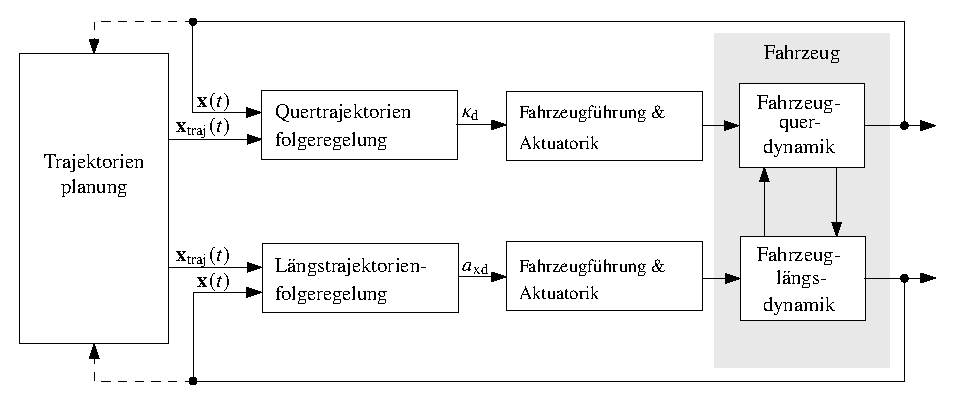
\includegraphics[width=12cm]{Bilder/04/2dof_bf.eps}
%	\caption{Anwendung der Zwei-Freiheitsgrade-Regelungsstruktur auf die Bahnführungsebene}
%	\label{abb_2dof_bf}
%\end{figure}

%Abb.  \ref{abb_2dof_bf} veranschaulicht die Anwendung der Struktur auf die Bahnführungsebene.  
Da die Trajektorienplanung durch Berücksichtigung des fahrdynamischen Potenzials die fahrdynamischen Grenzen und die Beschränkungen der verwendeten Aktuatorik berücksichtigt, kann die nachgelagerte Regelung in einen Quer- und Längsanteil aufgeteilt werden.
\subsection{Trajektorienfolgeregelung}
Ziel der Trajektorienfolgeregelung ist die Umsetzung der geplanten Trajektorie $\mathbf{x}_\mathrm{traj}(t)$ mit den Stellgrößen der Bahnführungsebene $\kappa_\mathrm{d}$ und $\aXD$.  Dabei wird auf die Zwei-Freiheitsgradestruktur gesetzt.  Diese wird zunächst kurz vorgestellt und anschließend auf die Quer- und Längsregelung angewandt.  
Die Zwei-Freiheitsgradestruktur ist eine häufig eingesetzte Methode zur Lösung von Trajektorienfolgeproblemen.  Abb. \ref{fig:2DOF} veranschaulicht die übliche Umsetzung.

\begin{figure}[htp!]
\centering
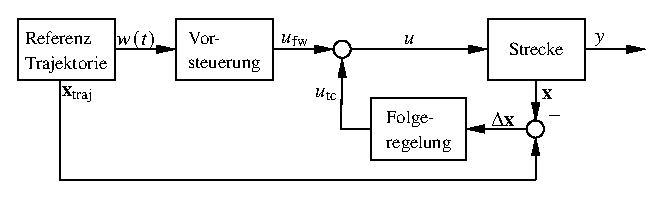
\includegraphics{Bilder/04/2DOF.eps}
\caption{Zwei-Freiheitsgrade-Regelungsstruktur}
\label{fig:2DOF}
\end{figure}

Es stehen sowohl der Zustandsverlauf der Trajektorie $\mathbf{x}_\mathrm{traj}$ als auch der gemessene Zustand $\mathbf{x}$ zur Verfügung.  Die unterlagerte Strecke wird durch die Dynamik $\tilde G$ und die Totzeit $T_\mathrm{D}$ beschrieben.  Entsprechend der Zwei-Freiheitsgrade-Regelung ergibt sich die Stellgröße $u$ mit 
\begin{equation}
u=u_\mathrm{fw}+u_\mathrm{tc}
\end{equation}
aus dem dominanten Vorsteuerungsanteil $u_\mathrm{fw}$ und dem Regelungsanteil $u_\mathrm{tc}$.  Ersterer hat die Aufgabe die unterlagerte Streckendynamik zu berücksichtigen und das Regelungsziel $w(t)$ bei Abwesenheit von Störungen zu realisieren:
\begin{equation}
u_\mathrm{fw} =  \tilde G^{-1} w(t+T_\mathrm{D})
\label{eq_u_ffw}
\end{equation}
Da die Trajektorie als Zustandsverlauf über der Zeit dargestellt ist, können bekannte Totzeiten direkt kompensiert werden indem die Trajektorie zur Berechnung der Führungsgröße zum um die Totzeit $T_\mathrm{D}$ prädizierten Zeitpunkt $t+T_\mathrm{D}$ ausgewertet wird.  

Da das Regelungsziel bereits zum Großteil durch die Vorsteuerung erreicht wird,  kann die Folgeregelung vergleichsweise einfach umgesetzt werden und auch eine Linearisierung des Systems entlang der Referenztrajektorie ist zulässig.  So wird die Stellgröße $u_\mathrm{tc}$ häufig durch Rückführung der Regelfehler $\Delta \mathbf{x} =  \mathbf{x}_\mathrm{traj}- \mathbf{x}$ mittels der Verstärkungsfaktoren $\mathbf{k}$:
\begin{equation}
u_\mathrm{tc} = \mathbf{k} \Delta \mathbf{x}
\end{equation}
berechnet.

Abb.  \ref{abb_zustaende_tfc} veranschaulicht die Zustände der geplanten Trajektorie sowie die gemessen Fahrzeugzustände.  
%
\begin{figure}[ht]
	\centering
	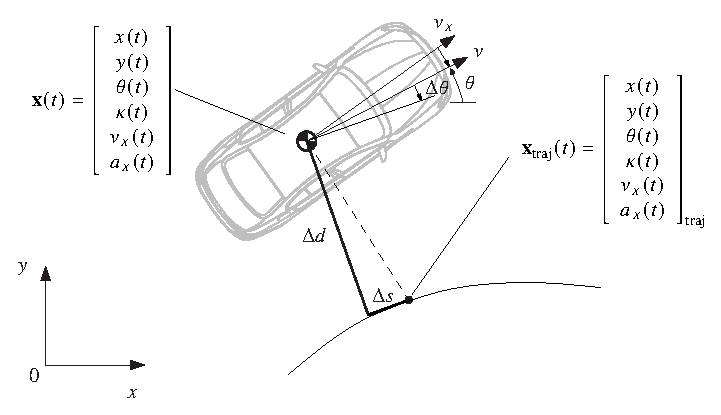
\includegraphics[width=0.9\textwidth]{Bilder/04/koordinaten_bahnfuehrung.eps}
	\caption{Darstellung der Zustandsgrößen der Trajektorenfolgeregelung}
	\label{abb_zustaende_tfc}
\end{figure}
%
In Querrichtung werden die Regelabweichungen zur geplanten Trajektorie über die Querablage $\Delta d$ und die Winkelabweichung $\Delta \theta$ und in Längsrichtung über den Längspositionsfehler $\Delta s$ und den Geschwindigkeitsregelfehler $\Delta v$ beschrieben:
\begin{equation}
\left[
\begin{matrix}
\Delta s \\ 
\Delta d \\ 
\Delta \theta \\ 
\Delta v_x
\end{matrix} 
\right]
:=
\left[
\begin{matrix}
\left[
\begin{matrix}
\cos \theta_\mathrm{traj} & \sin \theta_\mathrm{traj} \\ 
-\sin \theta_\mathrm{traj} & \cos \theta_\mathrm{traj} 
\end{matrix} 
\right]
\left[
\begin{matrix}
x_\mathrm{traj} -x\\ 
y_\mathrm{traj} -y
\end{matrix} 
\right]\\
\theta_\mathrm{traj} - \theta \\ 
\vXT- v_x.
\end{matrix} 
\right]
\label{eq_tfc_regelfehler}
\end{equation}
%
%
Der Kurswinkel $\theta$ ergibt sich dabei aus der Summe des Gierwinkels $\psi$ und Schwimmwinkels $\beta$.  Die Fehlerdynamik berechnet sich mit $v=\frac{v_x}{\cos{\beta}}$ zu
\begin{subequations}
\begin{align}
 \Delta \dot s &=  \vXT\kappa_\mathrm{traj} \Delta d + \vXT- v  \cos \Delta \theta \\
 \Delta \dot d &=   - \vXT\kappa_\mathrm{traj} \Delta s +  v \sin \Delta \theta \\
 \Delta \dot v_x &= \aXT- a_x \\
 \Delta \dot \theta &=  v _\mathrm{x,traj} \kappa_\mathrm{traj} - v \kappa\label{eq_dgl_theta}
\end{align}
\end{subequations}
%
Vernachlässigt man die Querfehler in der Bildung der Längsfehler und umgekehrt und betrachtet kleine Abweichungen, so erhält man die vereinfachten, linearen Gleichungen
\begin{subequations}
\begin{align}
 \Delta \dot s &=   \Delta v_x \\
 \Delta \dot d &=    v_x  \Delta \theta.
 \label{eq_dgl_d}
\end{align}
\end{subequations}
Diese stellen häufig die Grundlage für den Entwurf von linearen Spurführungsreglern dar (siehe z.B.  \cite{Ackermann1995}).
%
%
\subsubsection{Quertrajektorienfolgeregelung}
Entsprechend des in Kapitel \ref{ch_3EM} vorgestellten Drei-Ebenen-Modells ist als Stellgröße der Querregelung die Sollkrümmung $\kappa_\mathrm{d}$ definiert.  Die Dynamik der unterlagerten Regelung wird mit $\tilde G_{\kappa_\mathrm{d} \rightarrow \kappa }$ und der Totzeit $T_{\mathrm{D},\kappa}$ angenommen.  Entsprechend Gl.~(\ref{eq_u_ffw}) ergibt sich die Vorsteuerung der Quertrajektorienfolgeregelung zu
\begin{equation}
 \kappa_\mathrm{fw} = \tilde G_{\kappa_\mathrm{d} \rightarrow \kappa}^{-1}  \kappa_\mathrm{traj} (t+T_{\mathrm{D},\kappa}).
\end{equation}
Die Invertierung der Übertagungsfunktion kann mit den gängigen Methoden durchgeführt werden\footnote{Erfüllt die berechnete Trajektorie ausreichend Stetigkeitsanforderungen und kann so neben der Führungsgröße $\kappa_\mathrm{traj}(t)$ auch dessen Ableitungen bereitstellen, ist für die Invertierung der Streckendynamik kein Filter notwendig.}.\\
Die relevanten Regelfehler $\Delta d$ und $\Delta \theta$ lassen sich mit Gl.~(\ref{eq_tfc_regelfehler}) aus den gemessen und geplanten Zuständen berechnen.
Damit stehen alle notwendigen Informationen zur Verfügung und die Stellgröße der Querregelung berechnet sich zu
\begin{equation}
\kappa_\mathrm{d} = \kappa_\mathrm{fw} + \kappa_\mathrm{tc} = \tilde G_{\kappa_\mathrm{d} \rightarrow \kappa}^{-1}  \kappa_\mathrm{traj} (t+T_{\mathrm{D},\kappa})+ k_{\theta} \Delta \theta + k_d \Delta d
\end{equation}
mit den Verstärkungsfaktoren $k_{\theta}$ und $k_d$.  Die Verstärkungsfaktoren werden unter Zuhilfenahme der Bewegungsgleichen (\ref{eq_dgl_theta}) und (\ref{eq_dgl_d}) hergeleitet: Das Ziel von $\kappa_\mathrm{tc}$ ist es, Querabweichungen von der Zieltrajektorie asymptotisch zu unterdrücken: $\mathop {\lim }\limits_{t \to \infty } \Delta d(t) =0$.
Das Regelgesetz dazu resultiert unter Vernachlässigung der unterlagerten Dynamik direkt aus der Ableitung der Differenzialgleichung (\ref{eq_dgl_d}).  Durch dessen Ableitung erhält man
\begin{equation}
\Delta \ddot d = \dot v_x \Delta \theta + v_x \Delta\dot{{ \theta}} = a_x \Delta \theta - v_x^2 \kappa_\mathrm{tc}.
\end{equation}
%It has to satisfy a a second order homogeneous differential equation:
Fordert man als Wunschverhalten ein $PT_2$-Einschwingverhalten mit einer Wunschzeitkonstante $T_{\mathrm{tc},\kappa}$
%
\begin{equation}  
T_{\mathrm{tc},\kappa}^2 \Delta \ddot d + 2T_{\mathrm{tc},\kappa} \Delta \dot d + \Delta d = 0
\end{equation}
und löst nach dem Stellsignal $\kappa_\mathrm{tc}$ auf,  resultiert
\begin{equation}
\kappa_\mathrm{tc} = \Delta  \theta\, \underbrace{\frac{a_x T_{\mathrm{tc},\kappa}^2 + 2 v_x  T_{\mathrm{tc},\kappa}}{T_{\mathrm{tc},\kappa}^2 v_x^2}}_{k_\theta} + \Delta d \, \underbrace{\frac{1}{T_{\mathrm{tc},\kappa}^2 v_x^2}}_{k_d}.
\end{equation}
Dieses Regelgesetz garantiert das asymptotische Abklingen von Querablagefehlern\footnote{Um stationäre Genauigkeit zu erreichen,  muss der Kurswinkel korrekt erfasst werden.  Da der darin enthaltene Schwimmwinkel meist nur über einen Beobachter ermittelt wird,  kann bei nicht ausreichender Qualität ein zusätzlicher Beobachter auf Bahnführungsebene notwendig sein, vgl. \cite{Rathgeber2016}}.  Die Verstärkungsfaktoren sind geschwindigkeitsabhängig und stellen damit ein analytisches,  geschwindigkeitsabhängiges \textit{Gain Scheduling} dar. Unabhängig von der Fahrzeuggeschwindigkeit stellt sich das gleiche dynamische Verhalten des geregelten Systems ein.
\subsubsection{Längstrajektorienfolgeregelung}
Als Stellgröße der Längstrajektorienfolgeregelung ist die Sollbeschleunigung $\aXD$ definiert.  Die Dynamik der unterlagerten Regelung wird mit $\tilde G_{\aXD\rightarrow a_x }$ und der Totzeit $T_{\mathrm{D},a_x}$ angenommen. Die Längregelfehler $\Delta s$ und $\Delta v$ lassen sich entsprechend Gl.~(\ref{eq_tfc_regelfehler}) berechnen.  Damit ergibt sich das Regelgesetz
\begin{equation}
\aXD= a_{x,\mathrm{fw}} + a_{x,\mathrm{tc}} = \tilde G_{\aXD\rightarrow a_x}^{-1}  \aXT(t+T_{\mathrm{D},a_x})+ k_{v} \Delta v + k_s \Delta s
\end{equation}
mit den Verstärkungsfaktoren $k_v$ und $k_s$.  Diese werden analog zur Querregelung durch Forderung eines ideal gedämpften $PT_2$-Störunterdrückungs-Verhaltens mit der Zeitkonstante $T_{\mathrm{tc},a_x}$ berechnet und man erhält das Stellgesetz
\begin{equation}
a_{x,\mathrm{tc}} = \Delta v \underbrace{\frac{2}{T_{\mathrm{tc},a_x}}}_{k_v} + \Delta s \underbrace{\frac{1}{T_{\mathrm{tc},a_x}^2}}_{k_s}.
\end{equation}


\FloatBarrier
